%%%%%%% By Michał Swoboda
%%%%%%% Poprawki by Błażej Kowalczyk
%%%%%%% Uporządkował pewne rzeczy Bartłomiej Kurosz

\documentclass[xcolor=dvipsnames]{beamer}%[hyperref={pdfpagelabels=false}]{beamer}
\usepackage{lmodern}
\usepackage{polski}
\usepackage[utf8]{inputenc}
\usepackage{amsfonts}
\usepackage{tikz}
\usepackage{multicol}

%%%%%%%%%%%%%%%% Początek poleceń własnych
% Maksymalna dostępna wysokość pola w~prezentacji (między wąskim nagłówkiem a~stopką)
% dobrana eksperymentalnie - może w~przyszłości po prostu ją wyliczać???
\newlength{\maxheight}
\setlength{\maxheight}{\paperheight}
\addtolength{\maxheight}{-17.85pt}  % tyle zajmuje naczółek ze stopką 

% Polecenie do dokładania wycentrowanych rzeczy (zdjęć) na środku slajdu 
% bez tytulariów (ale ze stopką i~naczółkiem)
% By uzyskać obrazek "na całą stronę" jako argumentu należy użyć
% 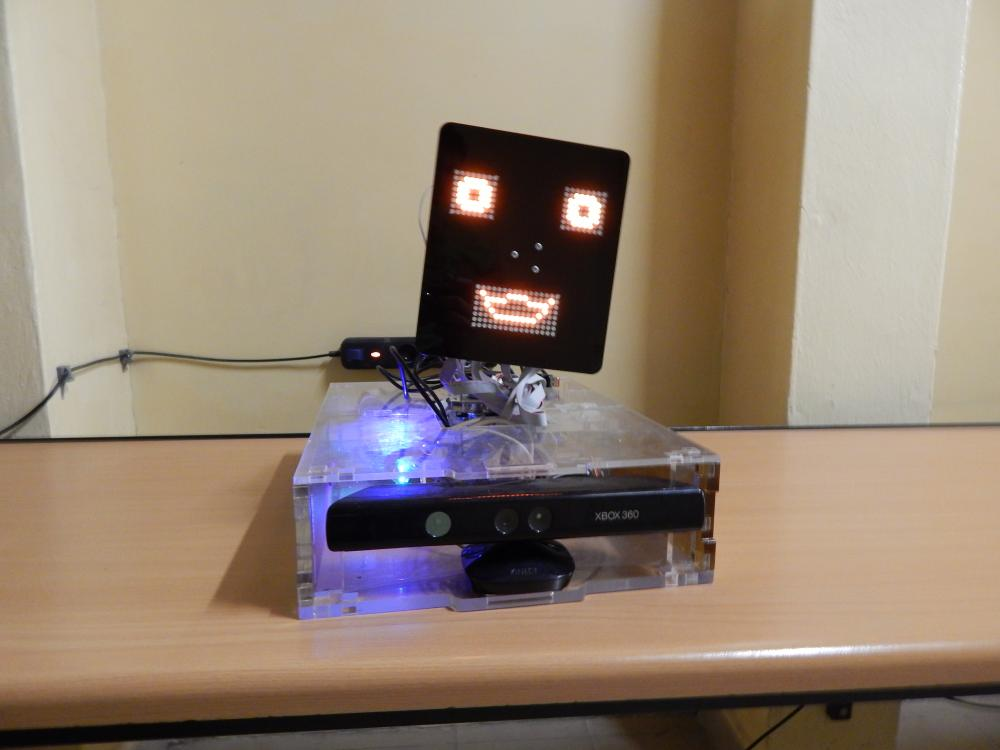
\includegraphics[height=\maxheight,width=\paperwidth]{figure/balbina.jpg}
% Jeśli nie chcesz zmian proporcji - zrezygnuj z~jednego z~wymiarów
% Obrazki za duże przykryją naczółek strony
% By wszystko było na swoim miejscu potrzebna jest dwukrotna kompilacja 
\newcommand{\framecentered}[1]{
  \setbeamertemplate{background canvas}{}
  \begin{frame}[c]
    \begin{tikzpicture}[overlay, remember picture]
      \node[anchor=center] at (current page.center) 
      {#1};
    \end{tikzpicture}
  \end{frame}}
%%%%%%%%%%%%%%%% Koniec poleceń własnych

%%%%%%%%%%%%%%%%Początek ustawień
\usebackgroundtemplate{%
  
\includegraphics[width=\paperwidth,height=\paperheight]{background/tlo_bezlogo.pdf}} 

\usepackage{beamerthemesplit}
\useoutertheme{infolines}
\useinnertheme{rounded}

\definecolor{konar2}{RGB}{240,152,52}
\definecolor{konar}{RGB}{151,58,66}

\setbeamercolor{block title}{fg=black,bg=konar2}
\setbeamercolor{block title alerted}{fg=konar2,bg=black}

\setbeamertemplate{navigation symbols}{}
\setbeamercolor{frametitle}{fg=white,bg=konar}
\setbeamercolor{section in head/foot}{bg=konar}
\setbeamercolor{author in head/foot}{fg=Black,bg=konar2}
\setbeamercolor{date in head/foot}{fg=Black}
\setbeamercolor{title in head/foot}{fg=white, bg=konar}
\setbeamercolor{section in head/foot}{fg=white}
\setbeamercolor{titlelike}{fg=black}
\setbeamercolor{structure}{bg=black, fg=konar2}
\setbeamercolor{subsection in head/foot}{fg=black}
\setbeamercolor{item}{bg=white}

%%%%%%%%%%%%%%%%%Koniec Ustawień

%%%%%%%%%%%%%%%%% SLAJD TYTUŁOWY

\title[Sonar z mikrofonami MEMS]{Wieloodbiornikowy czujnik ultradźwiękowy z mikrofonami MEMS} %tytuł prezentacji, skrócony w razie za długiej nazwy nie mieszczącej się w stopce
\author[Krystian Mirek]{Krystian Mirek} %autor, skrócony autor w razie za długiej nazwy nie mieszczącej się w stopce
\institute[ ]{promotor dr. Bogdan Kreczmer \and Wydział Elektroniki Fotoniki i Mikrosystemów \and Politechnika Wrocławska}
\date{\today}  %data

%%%%%%%%%%%%%%%%%



\begin{document}

\begin{frame}
\titlepage
\end{frame} 

\begin{frame}
\frametitle{Plan prezentacji}
\tableofcontents
\end{frame}

\section{Wstęp}
\subsection{Cel i zakres pracy}
\begin{frame} %początek sladjdu
\frametitle{Cel pracy}
%\framesubtitle{Podnazwa slajdu} %Opcjonalnie

 
Celem pracy jest konstrukcja sonaru pozwalającego wyznaczyć 
odległość do miejsca odbicia sygnału oraz kierunku nadejścia sygnału. 
Pozwalać ma to tym samym na precyzyjną lokalizację obiektu.
\end{frame}%koniec slajdu

\begin{frame}
	\frametitle{Zakres pracy}
Zakres pracy obejmował:
	\begin{itemize}
	\item projekt schematu ideowego,
	\pause
	\item projekt obwodu drukowanego,
	\pause
	\item montaż podzespołów,
	\pause
	\item oprogramowanie mikrokontrolera.
\end{itemize}
\end{frame}


\section{Konstrukcja}
\subsection{Zasada działania}
\begin{frame}
	\frametitle{Zasada działania}
	\begin{figure}
		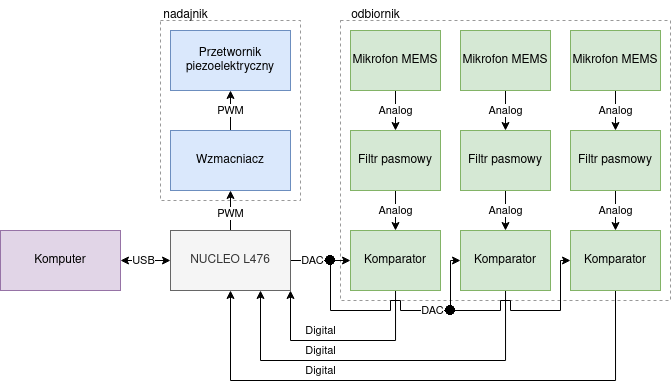
\includegraphics[width = \textwidth]{figure/sonar_uml.png}
	\end{figure}
\end{frame}

\subsection{Układ elektroniczny}
\begin{frame}
	\frametitle{Układ elektroniczny}
	\begin{figure}
		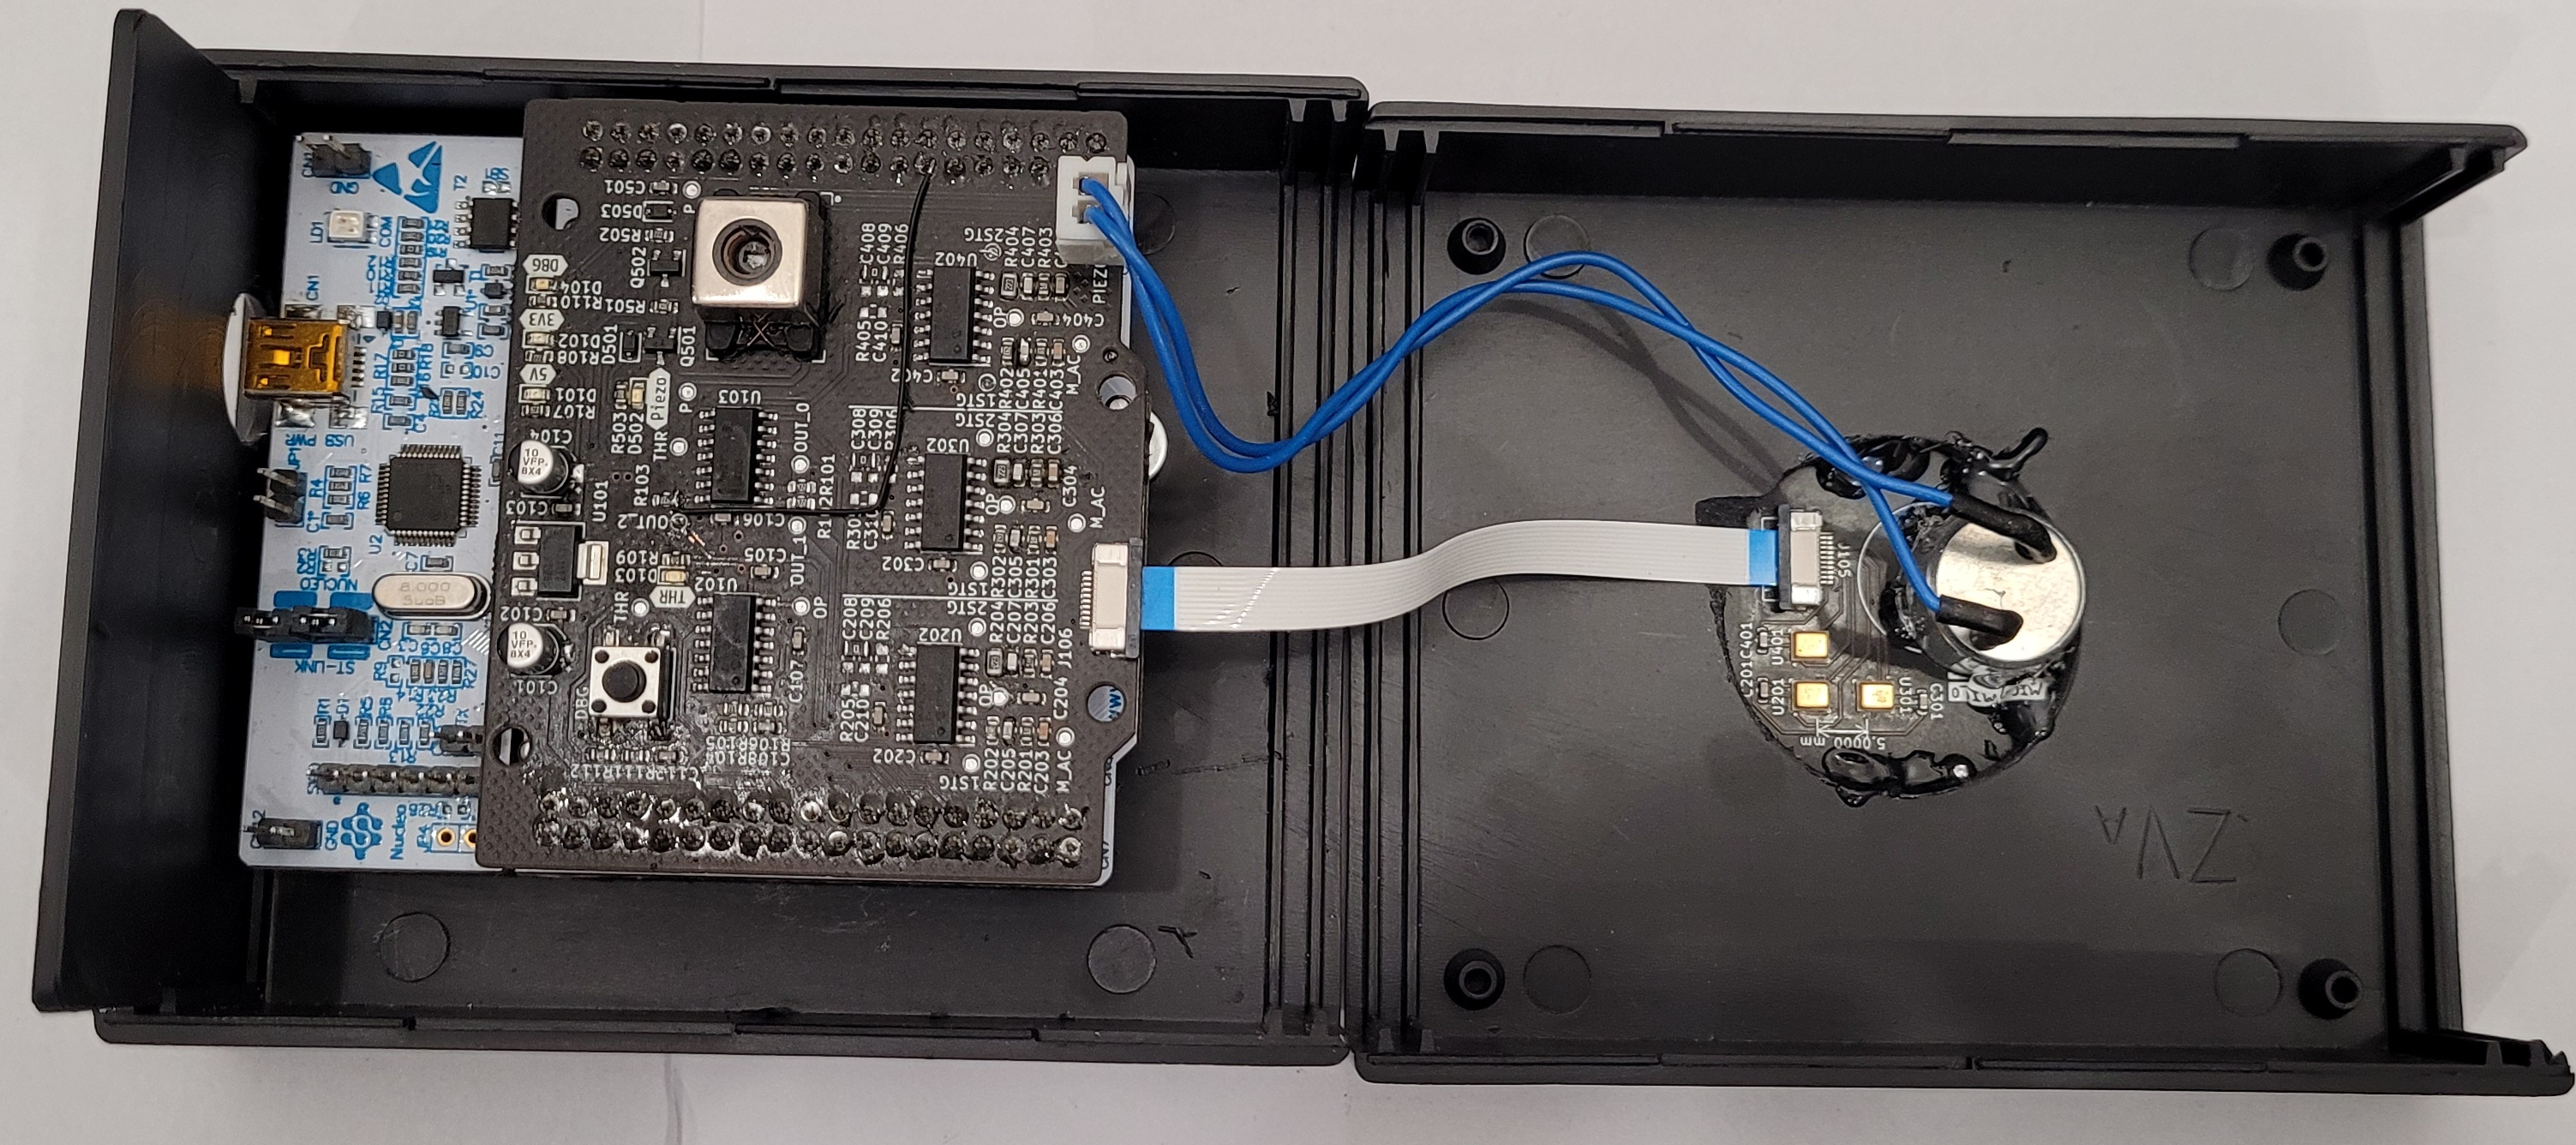
\includegraphics[width=\textwidth]{figure/doneotwarte.jpg}
	\end{figure}
\end{frame}

\subsection{Urządzenie}
\begin{frame}
	\frametitle{Urządzenie}
	\begin{figure}
		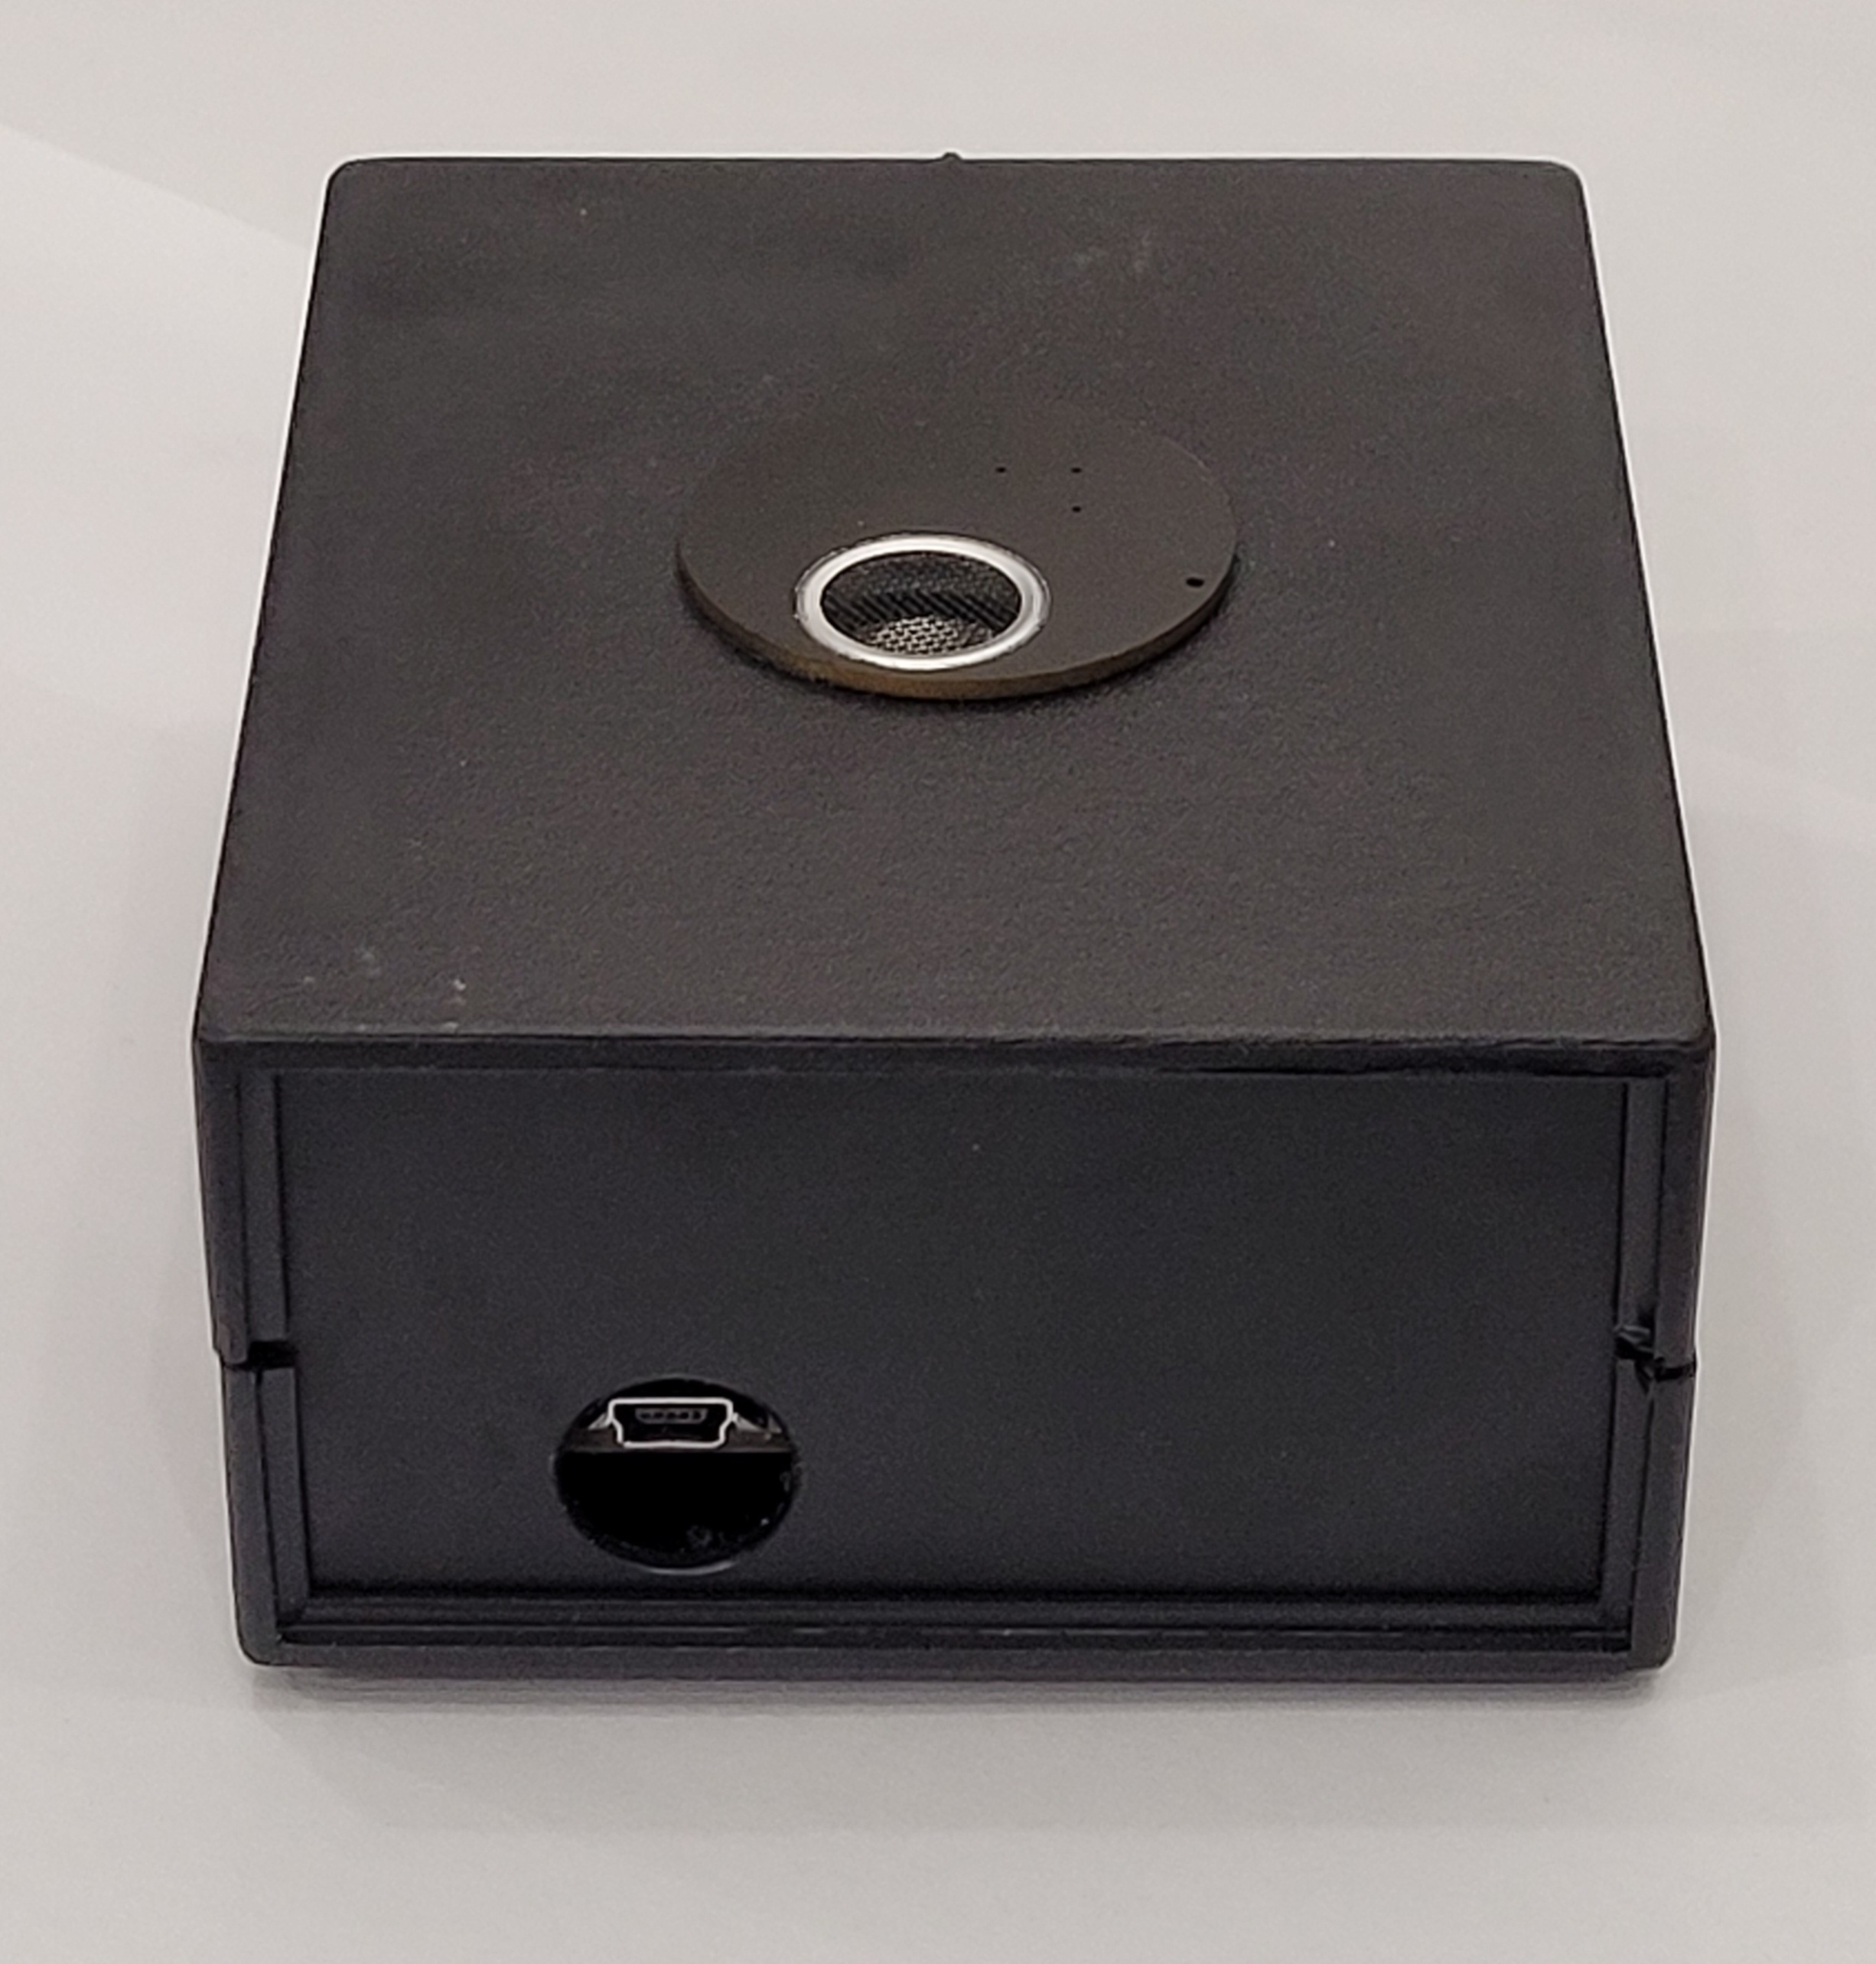
\includegraphics[width=0.6\textwidth]{figure/donezamkniete.jpg}
	\end{figure}
\end{frame}

\subsection{Komunikacja}
\begin{frame}
	\frametitle{Komunikacja}
	\begin{figure}
		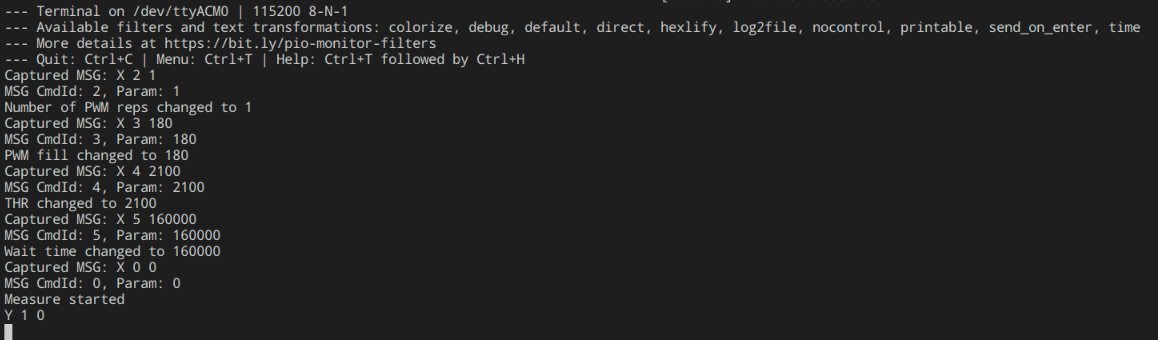
\includegraphics[width=\textwidth]{figure/comm.png}
	\end{figure}
\end{frame}

\section{Podsumowanie}
\subsection{Osiągnięte rezultaty}
\begin{frame}
	\frametitle{Interpretacja graficzna wykrycia obiektu}
	\begin{figure}
		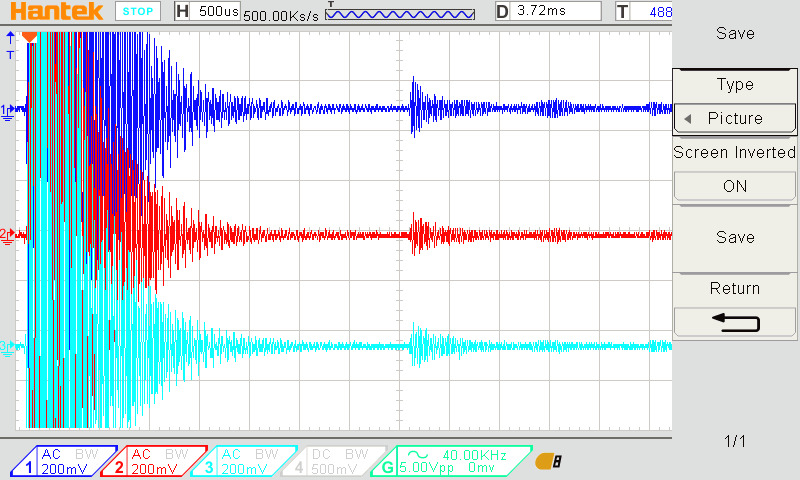
\includegraphics[width=\textwidth]{figure/dso_01_25_07_01_21.jpg}
	\end{figure}
\end{frame}
	
\begin{frame}
	\frametitle{Interpretacja graficzna położenia obiektu}
	\begin{columns}
		\begin{column}{0.49\textwidth}
			\begin{figure}
				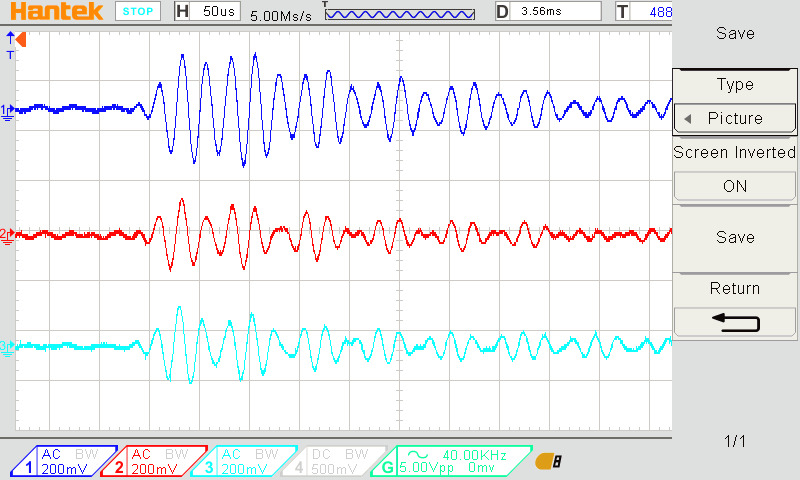
\includegraphics[width=\textwidth]{figure/dso_01_25_06_58_07.jpg}
				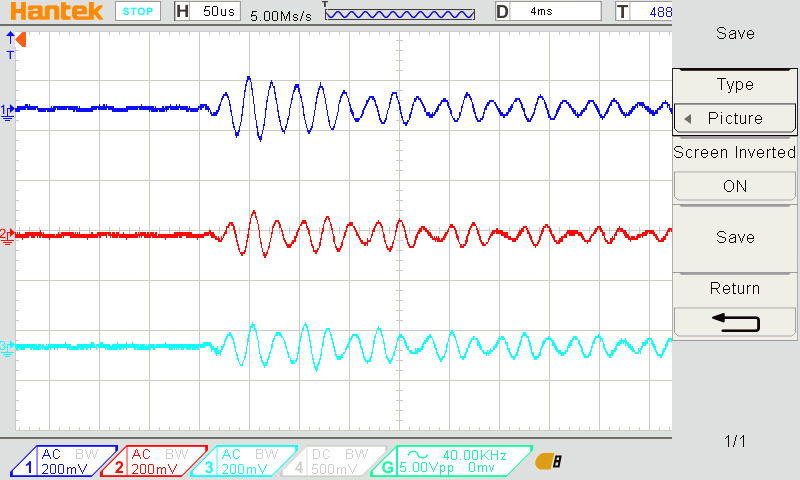
\includegraphics[width=\textwidth]{figure/dso_01_25_07_00_00.jpg}
			\end{figure}		
		\end{column}

		\begin{column}{0.49\textwidth}
			\begin{figure}
				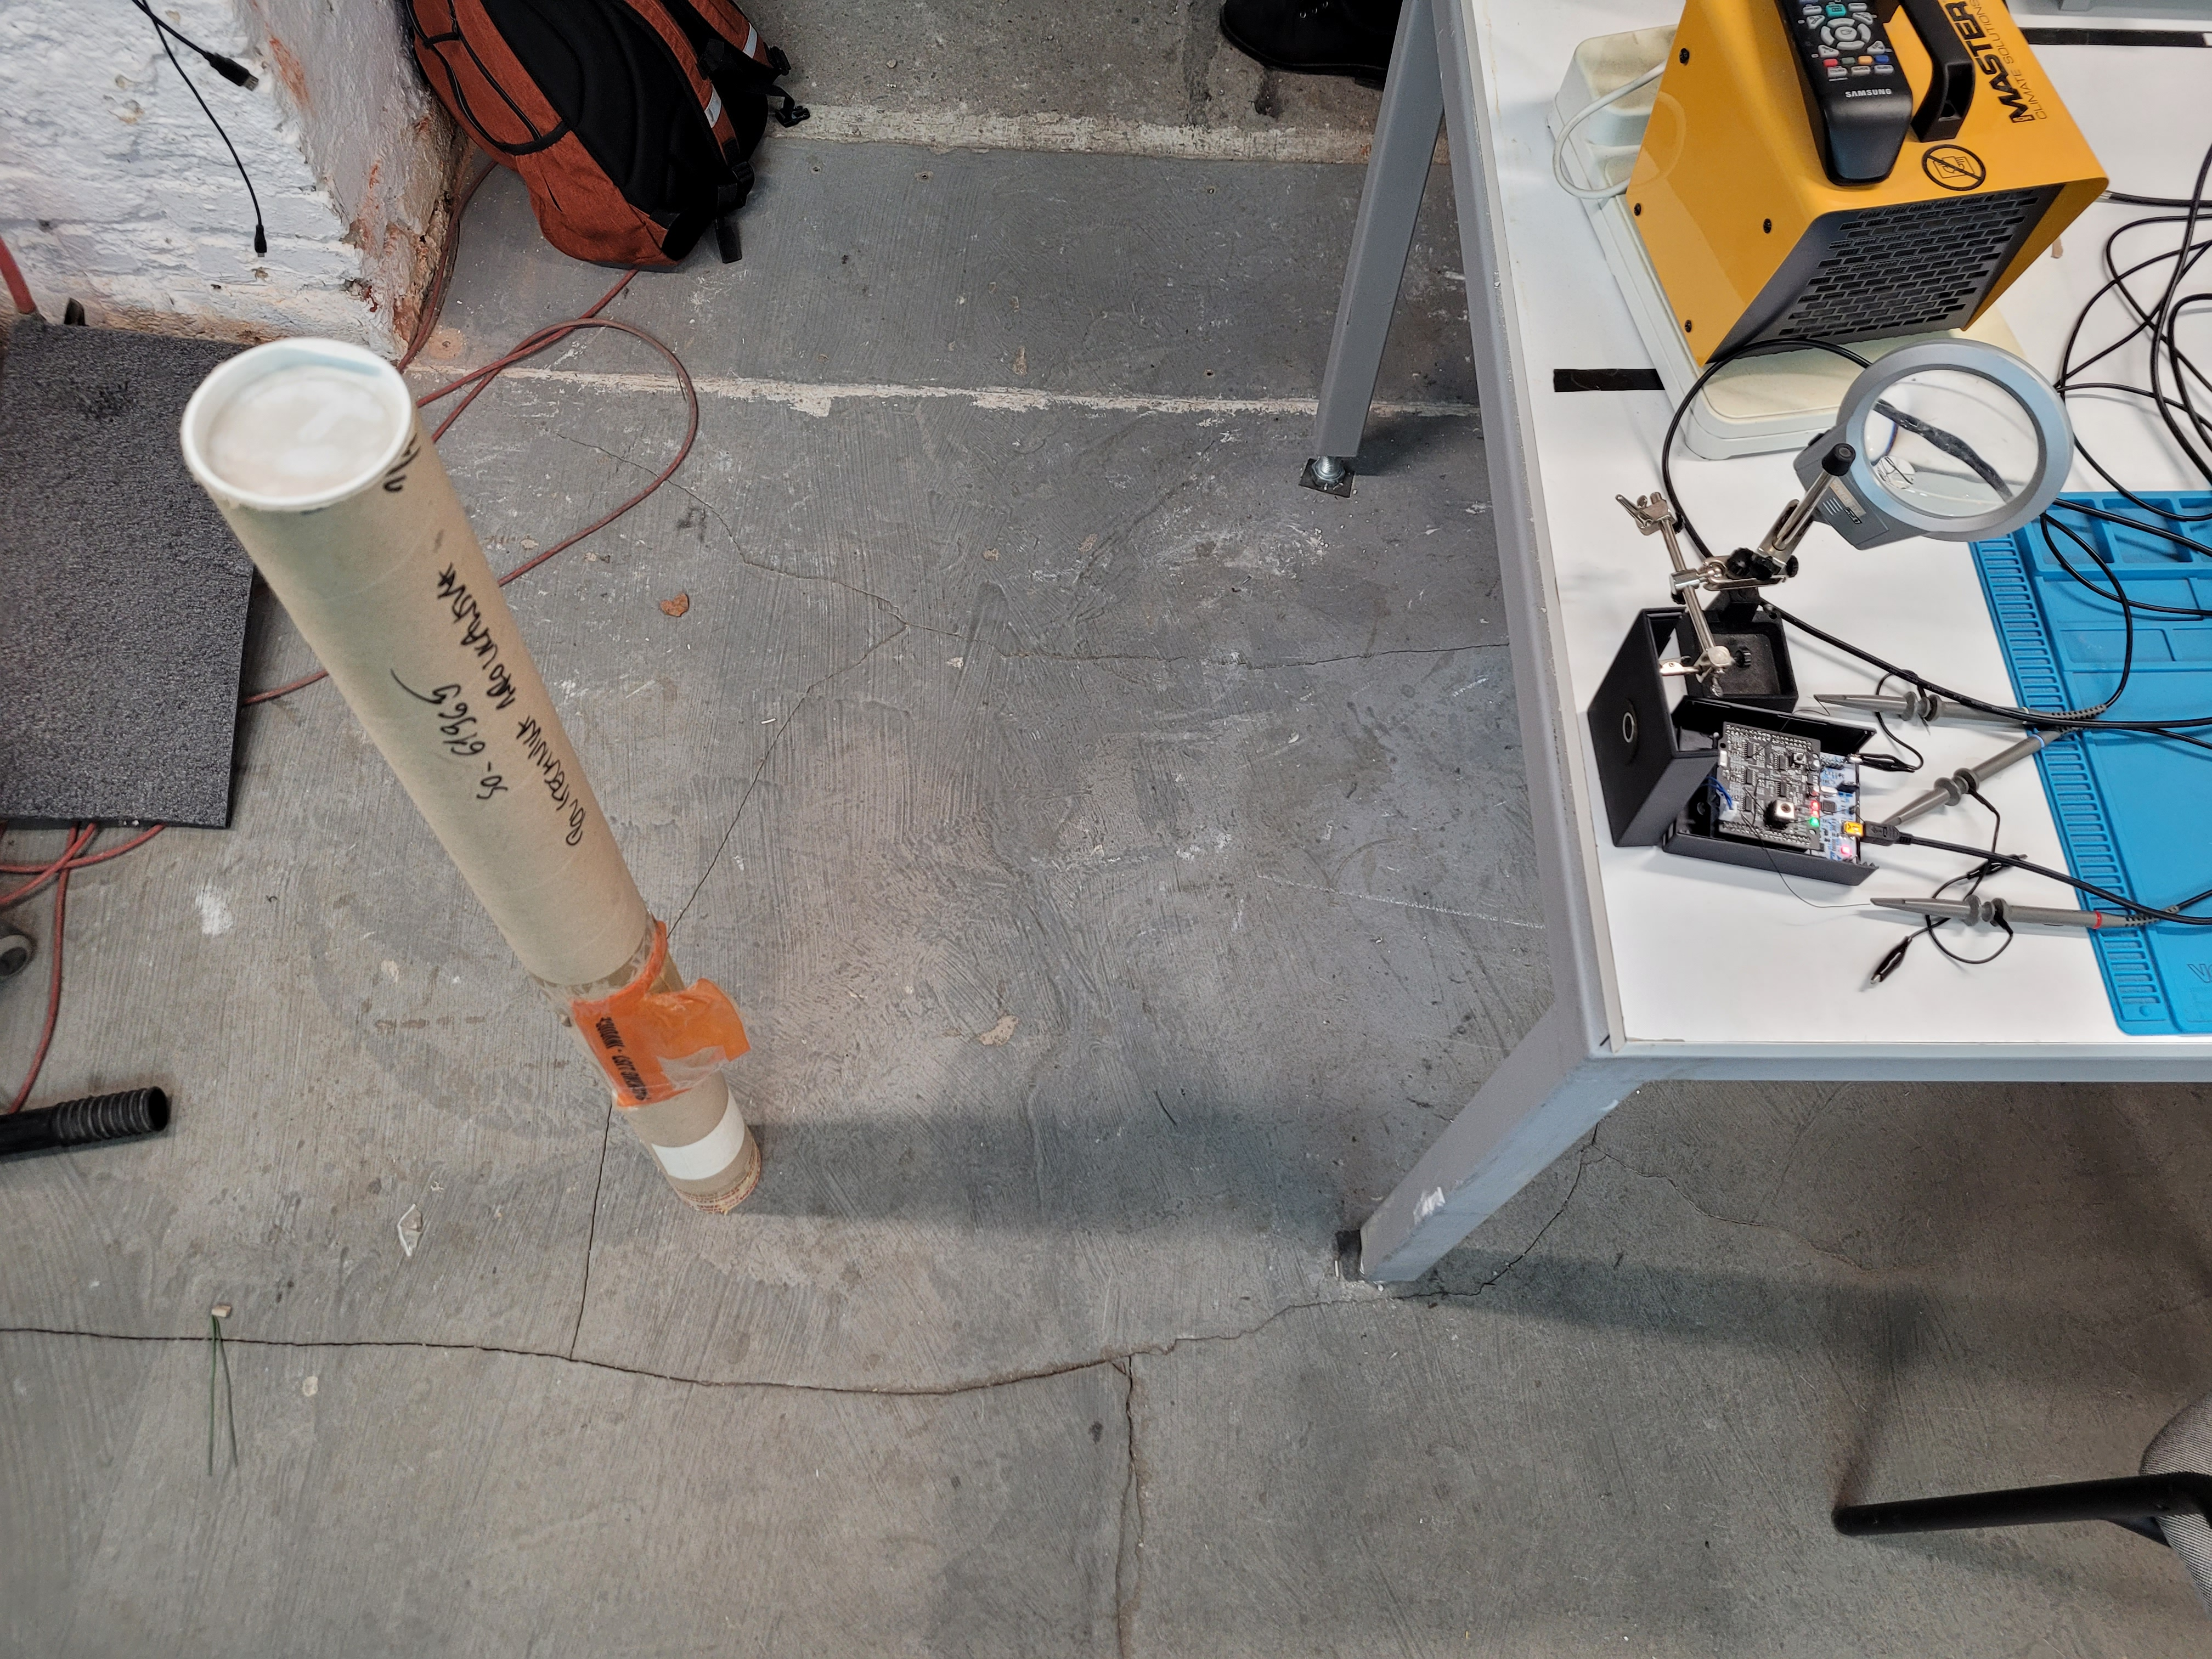
\includegraphics[width=0.8\textwidth]{figure/20230124_225325.jpg}
				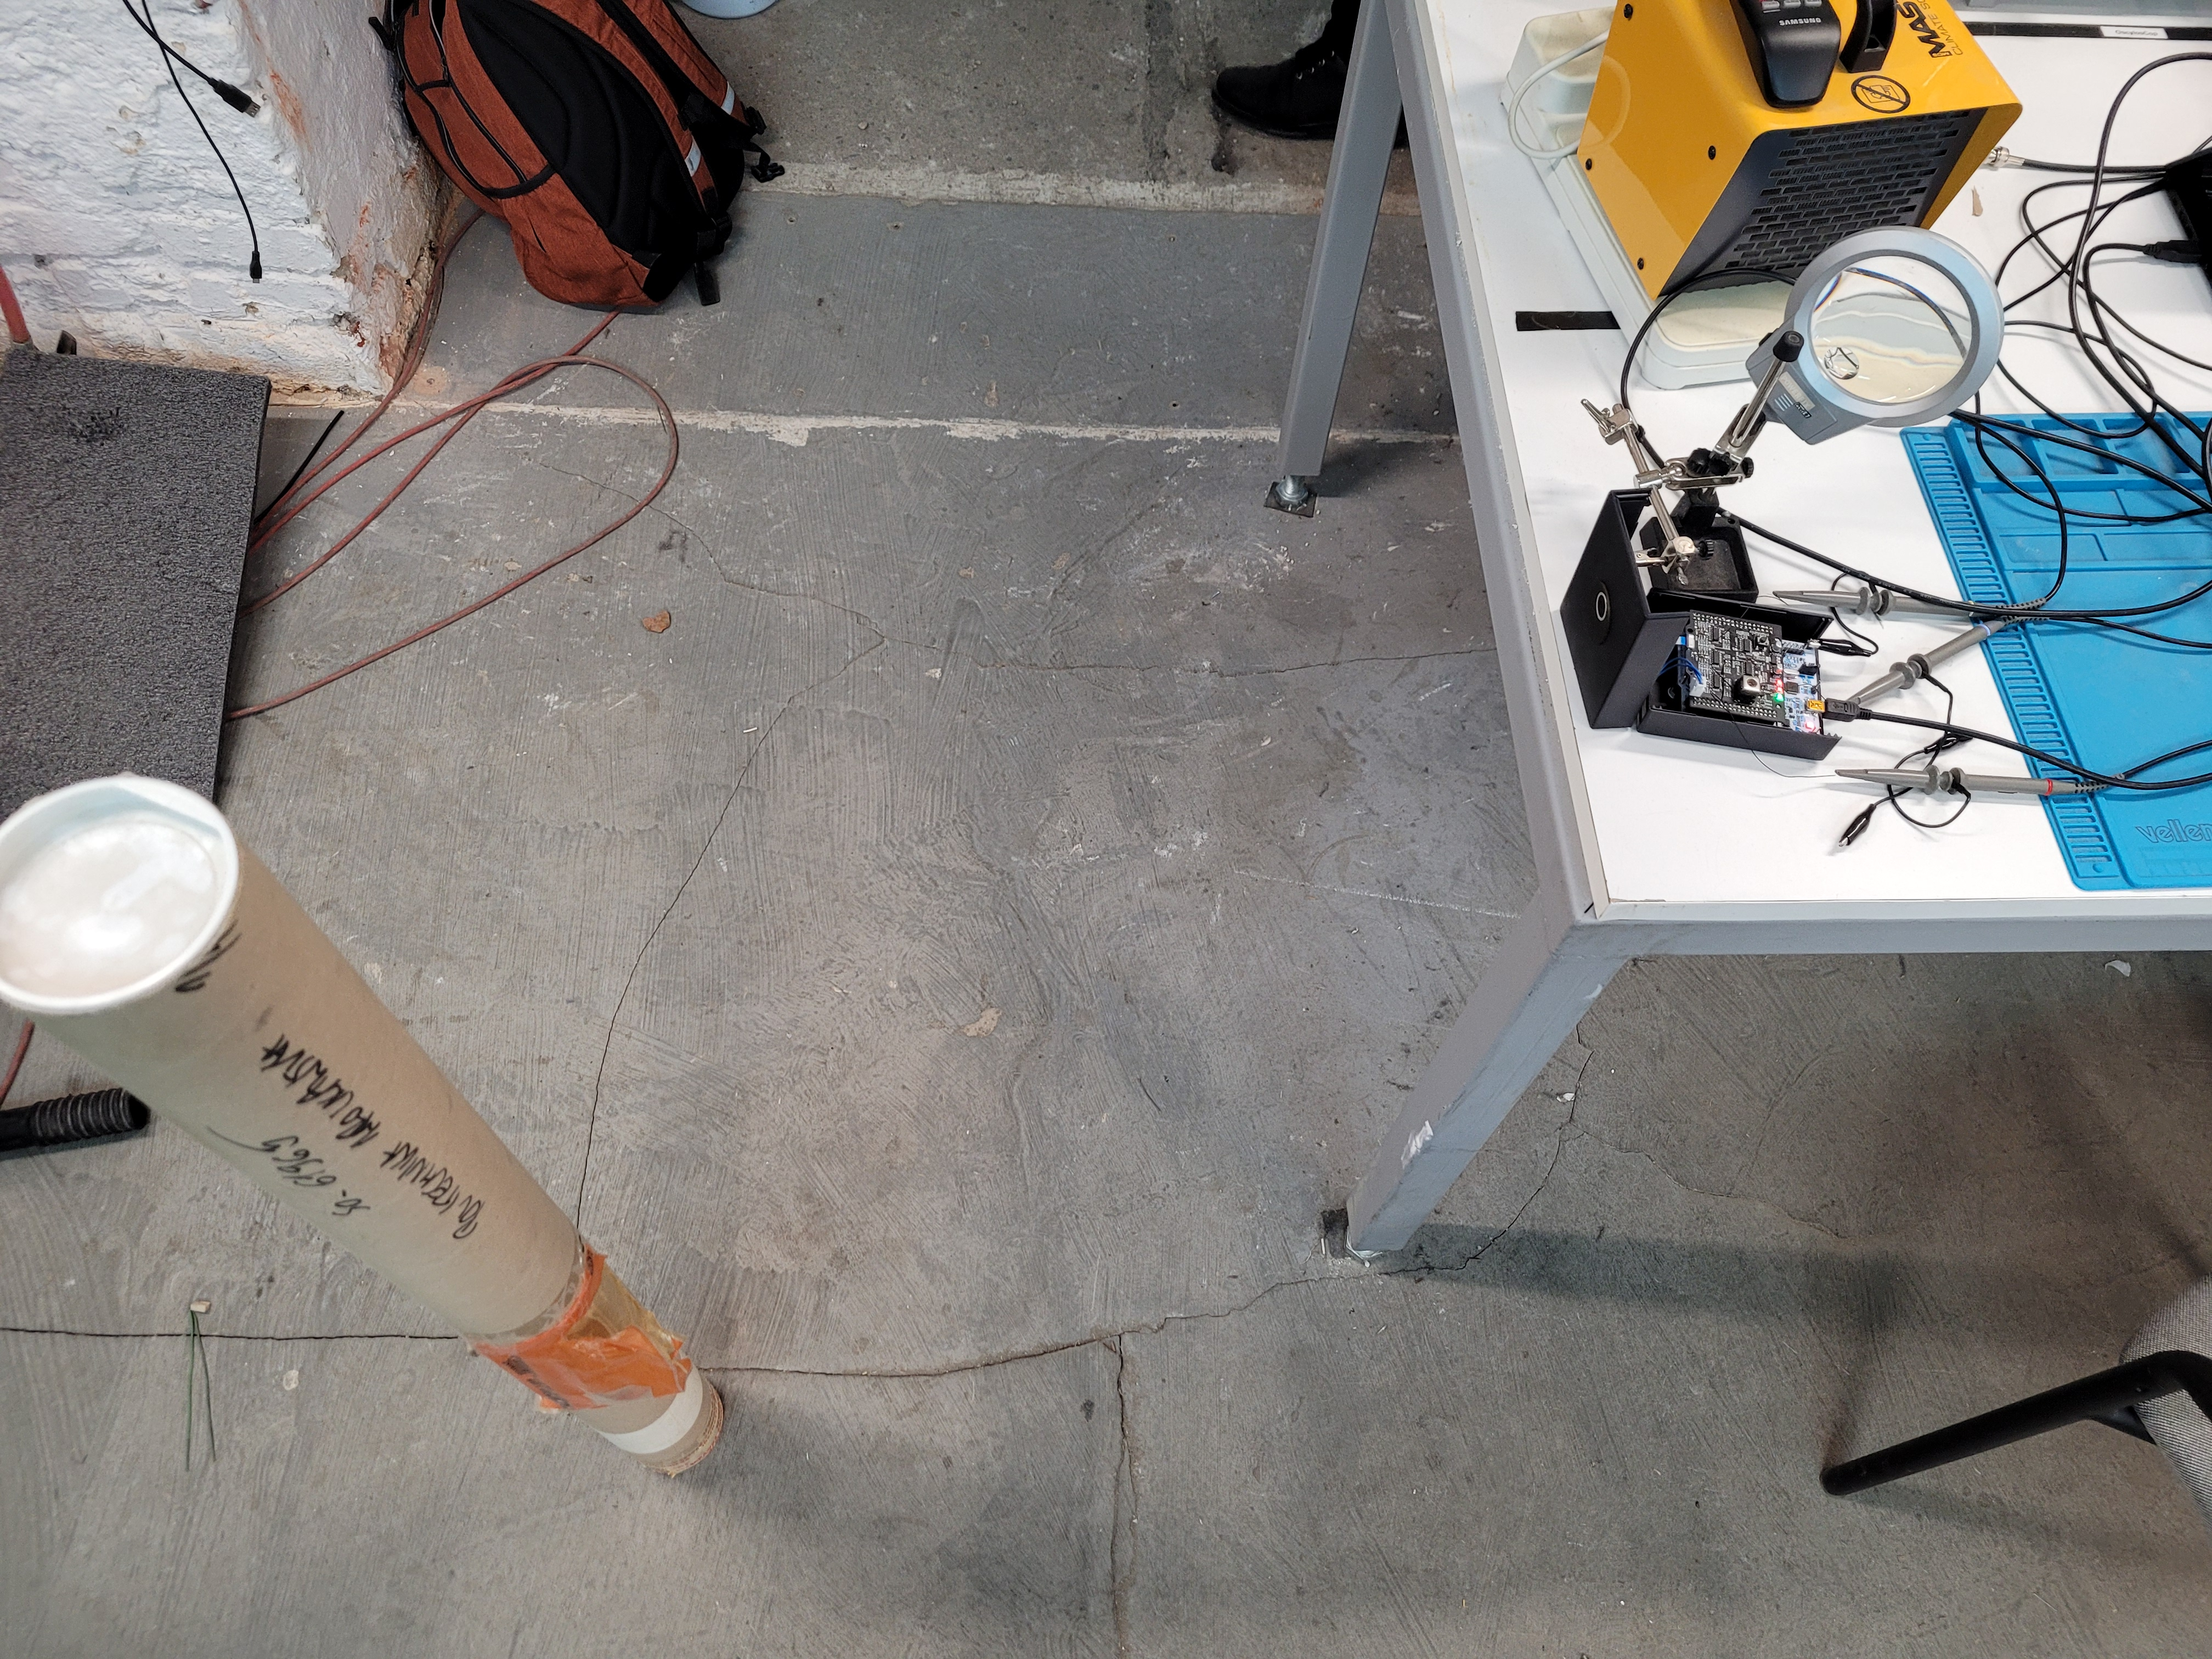
\includegraphics[width=0.8\textwidth]{figure/20230124_225339.jpg}
			\end{figure}		
		\end{column}
	\end{columns}
\end{frame}
	
\begin{frame}
	\frametitle{Interpretacja graficzna położenia obiektu}
	\begin{figure}
		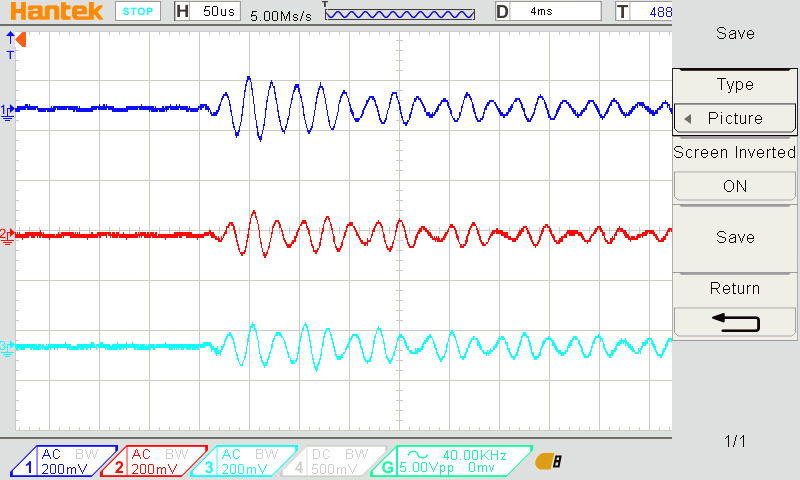
\includegraphics[width=\textwidth]{figure/dso_01_25_07_00_00.jpg}
	\end{figure}
\end{frame}

\begin{frame}
	\frametitle{Koniec}
	\centering
	Dziękuję za uwagę!
\end{frame}

\end{document}